%!TEX root=../document.tex
\section{Ergebnis}
\label{sec:Ergebnis}

Folgende Punkte wurden bearbeitet:


\begin{itemize}
	\item Allgemein
	\item CherryPy und andere angewendeten Technologien
	\item Vorgehensweise
	\item Aufgetretene Probleme	
	\item Ergebnis
\end{itemize}


\subsection{Allgemein}

Wir haben uns für CherryPy entschieden und für einen Anwendungsfall, der schnell zu implementieren und eine niedrige Komplexität aufweist. Das ist laut CherryPy einer der häufigsten Anwendungsfälle für CherryPy. Ein weiterer wichtiger Vorteil ist, dass CherryPy auf OOP ausgelegt ist und lässt sich dadurch zusätzlich leichter schreiben und verstehen.

Wir haben eine Webseite mit CRUD-Funktionen erstellt mit denen man Benutzer verwalten kann. 
Dazu haben wir in der Datenbank eine Tabelle angelegt die wie folgt ausschaut
\begin{figure}[!h]
\centering
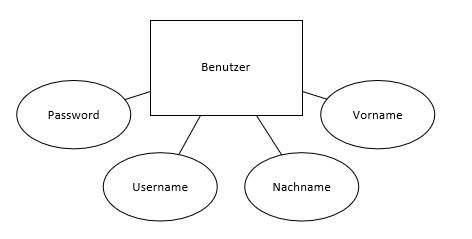
\includegraphics[width=0.5\linewidth]{images/db}
\caption{Aufbau von Benutzer}
\label{fig:Benutzeraufbau}
\end{figure}


Das Einsteigen in CherryPy ist mit Abstand einer der größten Vorteil, den mit wenigen Zeilen lässt sich eine Webseite erstellen und bereitstellen.
\begin{lstlisting}[language=Python]
import cherrypy

class HelloWorld(object):
@cherrypy.expose
def index(self):
return "Hello World!"

cherrypy.quickstart(HelloWorld())
\end{lstlisting}

Mit diesen Zeilen ist eine Webseite erstellt und bereit erweitert zu werden.

Insgesamt beläuft sich der Arbeitsaufwand auf ungefähr 0 Stunden.

\subsection{CherryPy und andere angewendeten Technologien}

CherryPy ist ein Non-Full-Stack-Framework und bietet mit einer sehr einfachen Verfahren einen Webserver an, der mit wenigen Befehlen gestartet und mit Inhalt gefüllt werden kann.

Weiters haben wir für unsere Persistierung die eingebaute Schnittstelle von Python zu SQLite verwendet. Dieses Schnittstelle ermöglicht es mit wenigen Befehlen eine simple Datenbank zu betreiben. Allerdings hatten wir auch einigen Probleme mit der Datenbank auf die wir später noch genauer eingehen.

Um die Webseite mit der CherryPy-Rückgaben zu verbinden, haben wir jQuery verwendet. 

Zusätzlich haben wir, um der Webseite ein sprechenden Design zu geben, CSS und Bootstrap verwendet. 


\subsection{Umsetzung}


\subsection{Aufgetretene Probleme}

\subsubsection{Tabelle nicht gefunden}
Die häufigste Fehlermeldung dieser Art war: $ no\,such\,table:\,benutzer $ 

Diesen Fehler konnten wir auf keine genaue Stelle eingrenzen, da dieser Fehler zufällig beim Starten des Server hin und wieder aufgetretten ist. 

Gelöst haben wir diesen Fehler dann durch das Sicherstellen, dass die Tabelle noch existiert und wenn nicht die Tabelle neu erstellt und mit Standarddatensätzen wieder befüllt wird.

\subsubsection{Datensatz nicht richtig abgespeichert}
Ein Fehler, der leicht zu lösen war, war: $ no\,such\,attribute:\,zuba $ 

Hierbei hat es sich um eine INSERT Anweisung gehandelt, die eine syntaktisch falschen Aufbau hatte, den wir allerdings erst sehr spät bemerkt haben. 

Gelöst haben wird dies, indem wir die Zusammensetzung der Anweisung neu geschrieben haben und explizit die Reihenfolge der Attribute angegeben haben.

\subsubsection{JS Funktionen nicht aufrufbar}$ function\,showuser\,not\,found $ 

\subsubsection{Aufrufprobleme}Delete konnte Daten nicht anzeigen, wenn davor Anzeigen aufgerufen wurde


\subsection{Ergebnis}
